\begin{figure}[htbp]
    \centering
    % The state vector is represented by a blue circle.
    % "minimum size" makes sure all circles have the same size
    % independently of their contents.
    \tikzstyle{state}=[circle,label=below:$r$,
                                        thick,
                                        minimum size=1.2cm,
                                        draw=blue!80,
                                        fill=blue!20]
    \tikzstyle{state2}=[circle,label=below:$e$,
                                        thick,
                                        minimum size=1.2cm,
                                        draw=blue!80,
                                        fill=blue!20]
    \tikzstyle{state3}=[circle,label=below:$a$,
                                        thick,
                                        minimum size=1.2cm,
                                        draw=blue!80,
                                        fill=blue!20]
    \tikzstyle{state4}=[circle,label=below:$d$,
                                        thick,
                                        minimum size=1.2cm,
                                        draw=blue!80,
                                        fill=blue!20]
    % The measurement vector is represented by an orange circle.
    \tikzstyle{measurement}=[circle,
                                                    thick,
                                                    minimum size=1.2cm,
                                                    draw=orange!80,
                                                    fill=orange!25]
     
    % The control input vector is represented by a purple circle.
    \tikzstyle{input}=[circle,
                                        thick,
                                        minimum size=1.2cm,
                                        draw=purple!80,
                                        fill=purple!20]
     
    % The input, state transition, and measurement matrices
    % are represented by gray squares.
    % They have a smaller minimal size for aesthetic reasons.
    \tikzstyle{matrx}=[rectangle,
                                        thick,
                                        minimum size=1cm,
                                        draw=gray!80,
                                        fill=gray!20]
     
    % The system and measurement noise are represented by yellow
    % circles with a "noisy" uneven circumference.
    % This requires the TikZ library "decorations.pathmorphing".
    \tikzstyle{noise}=[circle,
                                        thick,
                                        minimum size=1.2cm,
                                        draw=yellow!85!black,
                                        fill=yellow!40,
                                        decorate,
                                        decoration={random steps,
                                                                segment length=2pt,
                                                                amplitude=2pt}]
     
    % Everything is drawn on underlying gray rectangles with
    % rounded corners.
    \tikzstyle{background}=[rectangle,
                                                    fill=gray!10,
                                                    inner sep=0.2cm,
                                                    rounded corners=5mm]
     
    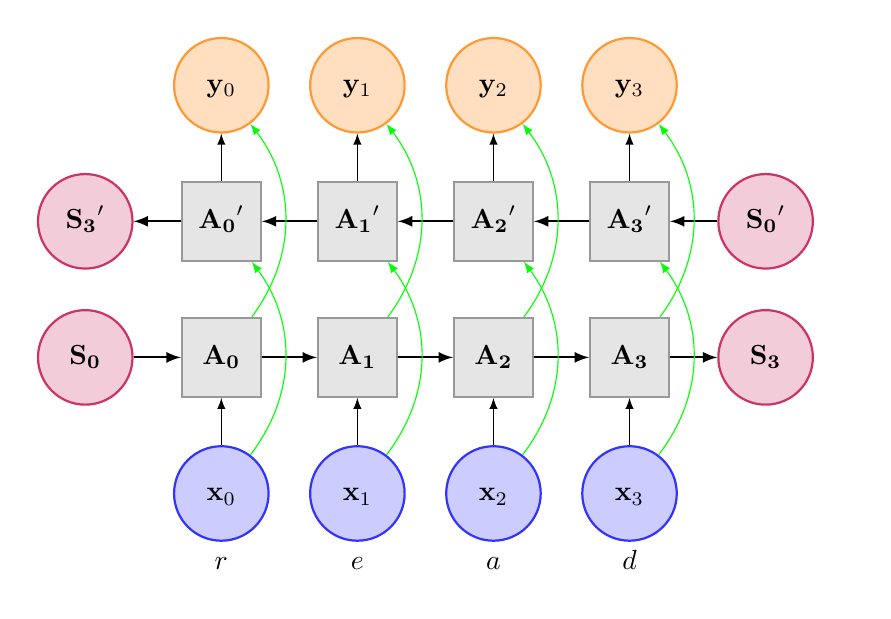
\begin{tikzpicture}[>=latex,text height=1.5ex,text depth=0.25ex]
        % "text height" and "text depth" are required to vertically
        % align the labels with and without indices.
     
      % The various elements are conveniently placed using a matrix:
      \matrix[row sep=0.5cm,column sep=0.5cm] {
        % First line: Control input
        &
        \node (y_0) [measurement] {$\mathbf{y}_{0}$}; &
    \node (y_1) [measurement] {$\mathbf{y}_{1}$}; &
    \node (y_2) [measurement] {$\mathbf{y}_{2}$}; &
            \node (y_3) [measurement] {$\mathbf{y}_{3}$}; &
            \\
            % Second line: System noise & input matrix
            \node ({S_{3}}') [input] {$\mathbf{S_{3}}'$}; &
            \node ({A_{0}}') [matrx] {$\mathbf{A_{0}}'$}; &
            \node ({A_{1}}') [matrx] {$\mathbf{A_{1}}'$}; &
            \node ({A_{2}}') [matrx] {$\mathbf{A_{2}}'$}; &
            \node ({A_{3}}') [matrx] {$\mathbf{A_{3}}'$}; &
         \node ({S_{0}}') [input] {$\mathbf{S_{0}}'$}; &
            \\
            \node ({S_{0}}) [input] {$\mathbf{S_{0}}$}; &
            \node ({A_{0}}) [matrx] {$\mathbf{A_{0}}$}; &
            \node ({A_{1}}) [matrx] {$\mathbf{A_{1}}$}; &
            \node ({A_{2}}) [matrx] {$\mathbf{A_{2}}$}; &
            \node ({A_{3}}) [matrx] {$\mathbf{A_{3}}$}; &
         \node ({S_{3}}) [input] {$\mathbf{S_{3}}$}; &
            \\
            % Fifth line: 输入
             &
            \node (x_0) [state]{$\mathbf{x}_{0}$}; &
     
             \node (x_1) [state2]{$\mathbf{x}_{1}$}; &
     
            \node (x_2)   [state3]{$\mathbf{x}_{2}$}; &
     
            \node (x_3) [state4]{$\mathbf{x}_{3}$}; &
     
        \\
        };
     
        % The diagram elements are now connected through arrows:
        \path[->]
            ({S_{0}}') edge[thick] ({A_{3}}')
            ({A_{3}}') edge[thick] ({A_{2}}')
            ({A_{2}}') edge[thick] ({A_{1}}')
            ({A_{1}}') edge[thick] ({A_{0}}')
            ({A_{0}}') edge[thick] ({S_{3}}')
     
            ({S_{0}}) edge[thick] ({A_{0}})
            ({A_{0}}) edge[thick] ({A_{1}})
            ({A_{1}}) edge[thick] ({A_{2}})
            ({A_{2}}) edge[thick] ({A_{3}})
            ({A_{3}}) edge[thick] ({S_{3}})
     
            (x_0) edge ({A_{0}})
            (x_1) edge ({A_{1}})
            (x_2) edge ({A_{2}})
            (x_3) edge ({A_{3}})
            ({A_{0}}') edge (y_0)
            ({A_{1}}') edge (y_1)
            ({A_{2}}') edge (y_2)
            ({A_{3}}') edge (y_3)
     
            (x_0) edge[->,bend right=37,green]	({A_{0}}')
            (x_1) edge[->,bend right=37,green]	({A_{1}}')
            (x_2) edge[->,bend right=37,green]	({A_{2}}')
            (x_3) edge[->,bend right=37,green]	({A_{3}}')
            ({A_{3}}) edge[->,bend right=37,green]	(y_3)
            ({A_{2}}) edge[->,bend right=37,green]	(y_2)
            ({A_{1}}) edge[->,bend right=37,green]	(y_1)
            ({A_{0}}) edge[->,bend right=37,green]	(y_0)
            ;
     
        % Now that the diagram has been drawn, background rectangles
        % can be fitted to its elements. This requires the TikZ
        % libraries "fit" and "background".
        % Control input and measurement are labeled. These labels have
        % not been translated to English as "Measurement" instead of
        % "Messung" would not look good due to it being too long a word.
     
     
    \end{tikzpicture}
     
    \caption{Kalman filter system model}
    \end{figure}
    